\section{El Concepte de 3BLD}

Per començar cal entendre el funcionament d'una resolució de blind, primer el cub és barrejat per una persona i el posa dins d'una capsa o un cube cover\footnote{Un cube cover és una tapa per cubs feta de cartró i que s'utlitza a les competicions}, després es col·loca a la taula boca avall i la persona que l'ha de resoldre es pren el seu temps per respirar. 
Un cop fet això la persona que resol el cub encén el timer i destapa el cub, de manera que el temps comença a comptar i es comença a memoritzar. Un cop acabada la memorització el que resol el cub es tapa els ulls amb un antifaç i comença a resoldre el cub, mentre que una persona externa li posa una cartiluna entre el cub i la seva cara per evitar trampes i mirar per sota de l'antifaç.
Tots aquests passos s'han d'executar perfectament per asegurar-se de la resolució compti.

\begin{figure}[ht]
    \centering
    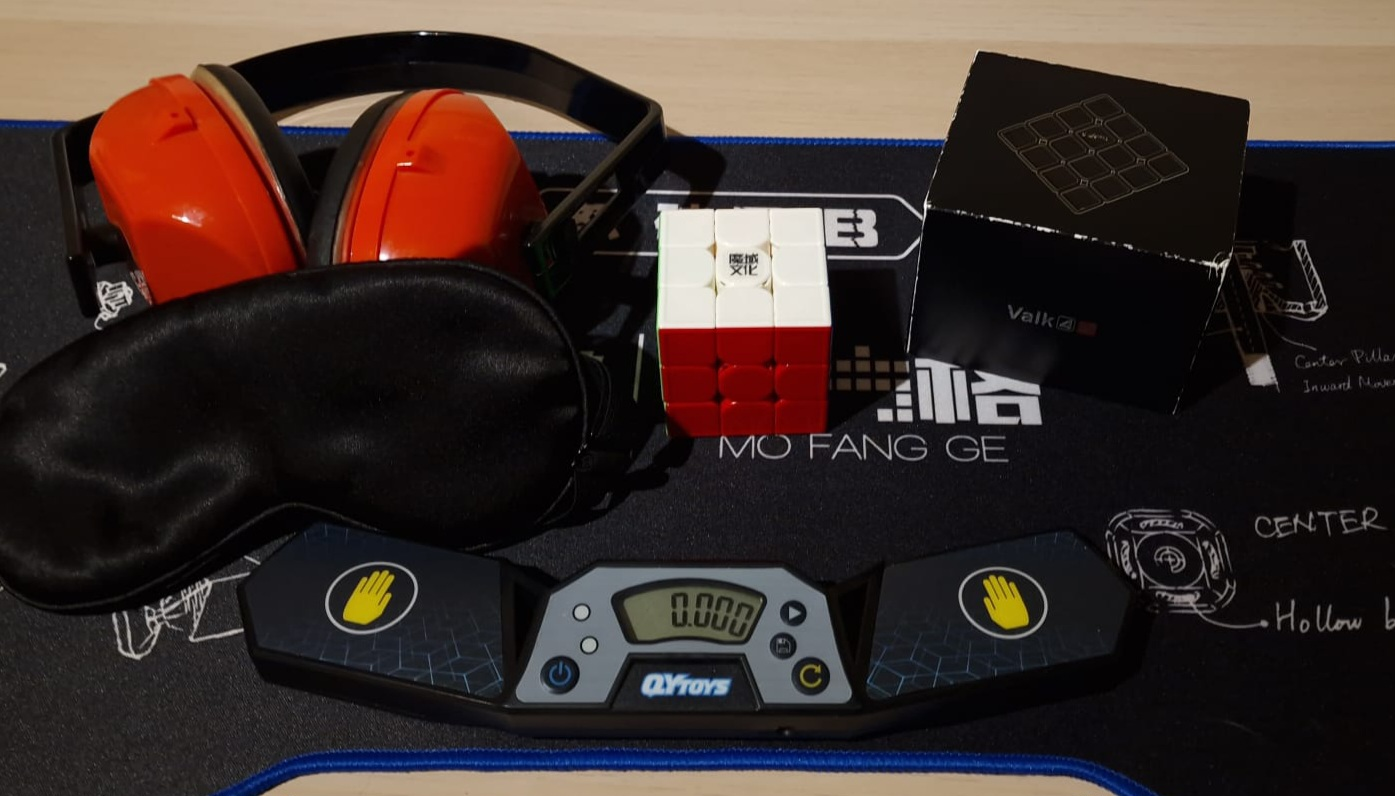
\includegraphics[width=12cm]{img/figures/materials-bld.jpg}
\caption{Materials necessaris per poder executar blind}
    \label{fig:materials-bld}
\end{figure}


\vspace{0.5cm}
\subsection{Fases de la Resolució}

Com ja he esmentat a la seccio anterior, completar el cub de Rubik amb els ulls tancats, es divideix en dos grans fases, memorització i execució. I dins d'aquestes fases hi han diferents procediments per poder aconseguir fer-ho correctament.

\subsection{Memorització}


En aquesta fase com ja ho diu el seu nom has de memoritzar el cub. La manera de memoritzar no és la més convencional ja que no memoritzes color sinó peces i com que hem d'interpretar el cub  com si fossin 20 peces el que fem es donar-li una lletra per la qual pots identificar a cada peça. Fent aquestes conversions has d'arribar a tenir el teu propi esquema de lletres, el que utilitzo jo és el de la figura \ref{fig:letter-scheme}, i el pots agafar com a plantilla per fer el teu o directament utilitzar-lo ja que si t'acostumes no et limitarà res durant el procés.

\begin{figure}[ht]
    \centering
    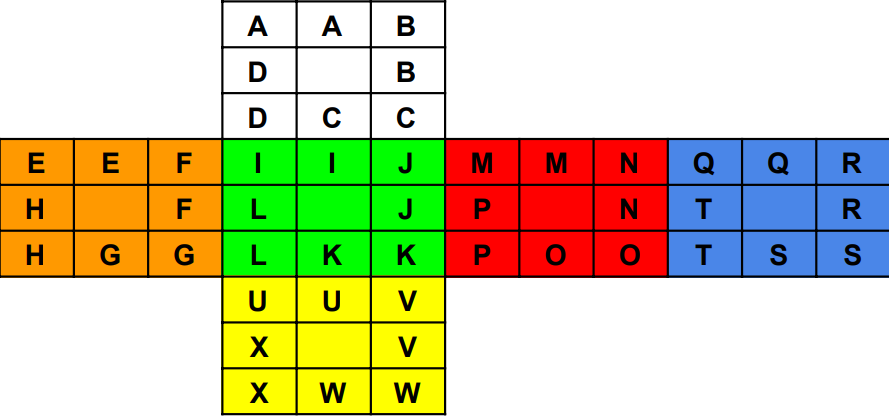
\includegraphics[width=12cm]{img/figures/letter-scheme.png}
\caption{Esquema de Lletres}
    \label{fig:letter-scheme}
\end{figure}

Hi han lletres repetides perquè primer memoritzes arestes i després cantonades, aquestes lletres a l'hora de memoritzar-les, no les memoritzes a força bruta, sinó que les converteixes en paraules que puguis convertir en imatges per poder entrecordar-te. Sembla molt complex però no ho és com es pot veure en el següent exemple.
Per practicar aquesta transformació d'imatges pots anar a la pàgina web \href{https://polsances13.github.io/roadto3bld/App.Html}{roadto3bld} on podràs veure el codi de la app i on hi haurà un link a github on podràs descarregar i utilitzar l'app.
\vspace{0.25cm}

$$ \textrm{Haig de memoritzar les lletres R i B    }  \rightarrow \textrm{   RedBull} $$
$$ \textrm{Haig de memoritzar les lletres A i C   }  \rightarrow \textrm{   Aire Acondicionat (AC és el símbol)} $$

Llavors has de tenir per a cada parell de lletres una paraula clau per memoritzarles ràpidament. Et pots inspirar en les d'algú però aquestes si que no les hauries de copiar, ja que aquestes paraules han de ser les que primer et vinguin al cap pensant en les dues lletres, és un treball una mica pesat però amb el temps dona el seu fruit.
No hi ha secret per integrar aquestes paraules a la teva ment, el que has de fer és practicar, practicar i practicar, i amb el temps et sortirà sol.


\subsection{Execució}

A diferència de una resolució normal, a l'hora d'executar els moviments tu no pots rotar el cub, perquè tens que actuar segons les lletres que has memoritzat i si rotes el cub canvies la posició de les peces respecte a les lletres indirectament. 
Per tant només fas moviments de les capes. Els algoritmes per intercanviar les peces només interfereixen en les lletres que has memoritzat i deixent la resta del cub exactament igual quan fas els passos. Per començar a fer el cub has d'aprendre el mètode principants que explicaré a la següent secció.
Durant l'execució se segueix l'ordre CEEC que diu que memoritzes cantonades, després arestes, executes arestes i després executes cantonades.
